\chapter{Teknologi}

\section{Indledning}
Realtidskommunikation via internettet er ikke længere blot en chatsamtale med en ven eller en telefonopringning via Skype. Teknologien giver i dag mulighed for, at sundhedsfagligt personale kan kommunikere med borgere på en måde, der for blot få år siden syntes utænkelig.\\Telesundhed er brugen af telekommunikationsteknologier til at levere sundhedsmæssige ydelser, såsom udveksling af patientdata, hjemmemonitorering og videokonferencer, hvor distance ofte er en væsentlig faktor.\\
Brugen af open source-software er stigende \footnote{Kilde 1}, hvilket har øget mængden af tilgængelig brugbar kode og dermed sat skub i udviklingen. \cite{hp2} og \cite{hp4}
\\
Appinux er en af spillerne på markedet, der med deres open source-baserede løsning, bl.a. giver mulighed for, at plejepersonalet kan kommunikere med borgere, der er tilknyttet systemet. Som konsekvens af den teknologiske udvikling opstår der nye problemstillinger, hvor bl.a. infrastruktur og patientsikkerhed er nøglebegreber, der sætter krav til behandlingen og ikke mindst overførsel af data. Dette teknologiafsnit ser nærmere på, hvilke forudsætninger, der skal være opfyldt for at videokonferencesystemer i telesundhed fungerer optimalt og undersøger, hvorledes Appinux står ift. disse.
\section{Metoder}
Dette afsnit bygger i høj grad på informationer fra en samtale med Appinux' salgdirektør Michael Ellegaard. Det har været været vanskeligt at finde litteratur, der direkte undersøger Appinux' løsning, så fokus har i stedet ligget på de delelementer og standarder, som Appinux anvender og bygger på. Der er deraf foretaget litteratursøgning på dette med henblik på at klarlægge både mangler og muligheder.
Metodeafsnit ikke færdiggskrevet.

\section{Komponenter i telesundhedsløsninger}
Flere telemedicinske initiativer i kommunerne befinder sig på et pilot- eller projektstadie og mange af disse projekter er ikke udrulleret i stor skala. Nogle kommuner iværksætter telemedicinske projekter uden at have telemedicinsk strategi liggende i skuffen. Det viser sig også at nogle disse projekt opløses efter noget tid, da det hverken forbedre eller effektivisere det ønskede område. Vellykket telemedicinsk projekter kræver ikke kun business cases, som fokusere på de økonomisk besparelse, der kan være i telemedicinske løsninger. Forudsætningen for et succesfuld udbredelse af telemedicin er derimod et helhedsstrategi, der tilgodeser de tekniske, faglige, organisatoriske og økonomiske forudsætninger i sådan en proces. I det følgende vil der blive behandlet de tekniske aspekter i telemedicin.\\
Tekniske forudsætninger for udbredelse af telemedicin kræver overordnet set et passende udstyr og en slags telekommunikationsmedium. Desuden kræver det en grundig forståelse af det man populært kalder for state-of-the-art, altså at have kendskab til det nyest og forskningsbaseret teknologier inden for telemedicin. Dette kendskab gør at man er velorienteret i området og ved hvornår man skal benytte ” commercial of-the-shelf” (COTS) teknologier for at minimere omkostningerne eller vælge at udvikle egne løsninger selv. Evnen til at kunne vælge de rigtige løsninger til de rigtige opgaver er en nøgle kompetence, når der skal indføres telemedicinske løsninger. De teknologiske forudsætninger som skal være opfyldt for at indføre telemedicin kan inddeles i tre kategorier\footnote{Telemedicine System Engineering. S.34}:
\begin{itemize}
\item Udstyr til at fange klinisk data på hver side
\item Udstyr, der viser data i hver side. 
\item Forbindelsen, som transmitterer data imellem udstyrene
\end{itemize}

Overstående punkter vil blive behandlet i det følgende.

\subsection{Udstyr til måling af medicinsk data kan inddeles i tre komponenter}

\begin{figure}[H]
	\centering
	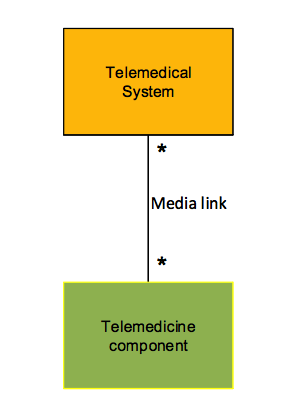
\includegraphics[width=1\textwidth]{Figurer/Snip20160504_29}
	\caption{Viser at telemedicinske systemer består af en eller flere telemedicinske komponenter}
\end{figure}

\begin{figure}[H]
	\centering
	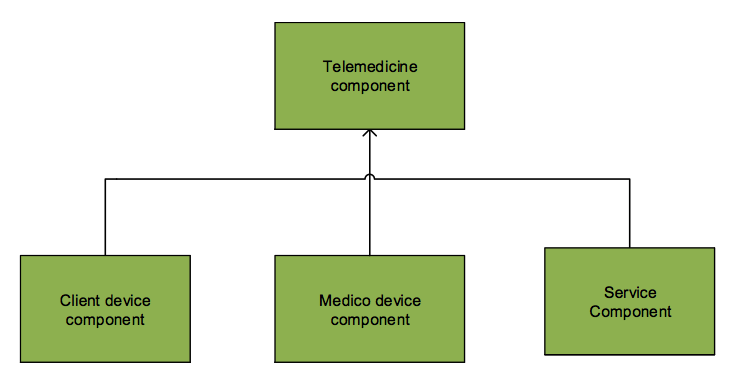
\includegraphics[width=1\textwidth]{Figurer/Snip20160504_30}
	\caption{Viser oversigt over de teknologier, der er brugt til at måle klinisk data}
\end{figure}

\subsection{Udstyr, der viser data i hver side}
\begin{figure}[H]
	\centering
	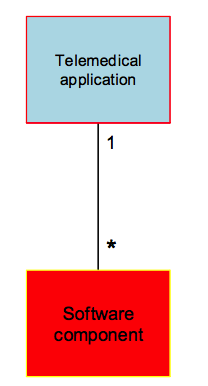
\includegraphics[width=0.2\textwidth]{Figurer/Snip20160504_31}
\end{figure}

\begin{figure}[H]
	\centering
	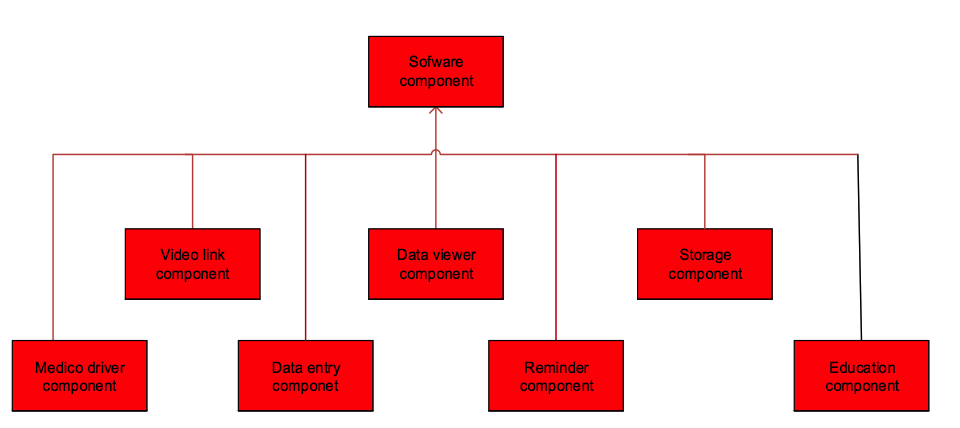
\includegraphics[width=1\textwidth]{Figurer/Snip20160504_32}
	\caption{Viser forskellige komponenter som telemedicinsk software kan bestå af.}
\end{figure}

\section{Resultater}
\subsection{Infrastruktur}
Telekommunikation som videokonferencesystemer, er afhængig af tilstedeværelsen af en  internetforbindelse.\\
En internetforbindelse er efterhånden blevet en selvfølge i Danmark. I 2015 havde 93\% af befolkningen i Region Midtjylland adgang til PC og internet i hjemmet\footnote{statistikbanken.dk}. Andelen af mobiltelefonbrugere mellem 16 og 74 år, der bruger mobiltelefonen til at tilgå nettet er ligeledes steget fra 9\% i 2008 til 63\% i 2013\footnote{\url{http://www.dst.dk/Site/Dst/Udgivelser/GetPubFile.aspx?id=18685&sid=itanv}}. Dette har ændret det digitale landkort i den forstand, at teleselskaberne, som leverer disse services må holde trit med udviklingen.\\ \\
Overordnet set vil denne MTV skelne mellem mobilt bredbånd og en kablet forbindelse, som inkluderer fiber-, coaxial- og kobberforbindelser, da det er her det største skel ift. videokonferencesystemer ligger.
Når man snakker om godt internet har hastigheden ofte været den faktor. Den mest udbredte opkoblingstype i Danmark er ADSL-bredbånd med over en million abonnementer i Danmark\footnote{\url{http://www.statistikbanken.dk/DIS122}}. Hastighed på disse ligger typisk fra x til x. Det har ikke været muligt at finde et dækningskort, der viser fiber- og bredbåndsdækningen i Favrskov Kommune, men som udgangspunkt må man forvente, at hvis en borger har købt bredbånd med en given hastighed, bliver produktet også leveret.\\
Mobilt bredbånd er kommet mere og mere i fokus, og med indførslen af 4G, er hastigheden også kommet op og minde om en bredbåndsforbindelse. Eftersom det hele kører trådsløs, er dækningen utrolig vigtig for, at et videokonferencesystem kører optimalt. TDC's dækningskort viser, at Favrskov Kommune har min. 5Mbit/s på enten 3G- eller 4G-netværket udendørs\footnote{\url{http://daekning.tdc.dk/tdcnetmap_ext_tile/Default/mobile}}. Det kan dog være svært at sige, hvorledes hastigheden stemmer overens indendørs, og det er dermed vigtigt at undersøge dette i hver given sitution. Der har været indberetninger fra borgere, der antyder, at der i kommunen i efteråret 2015 var problemer med mobildækningen indendørs\footnote{\url{http://www.tv2oj.dk/artikel/280010:Favrskov--Favrskov--Her-er-der-ringe-mobildaekning}}, hvilket har udmøntet sig sig et dækningskort\footnote{\url{http://favrskov.lokalavisen.dk/assets/pdf/PL1825408727.PDF}}, hvilket kan indikere, at problemet enten er løst eller der under bearbejdning.

\subsection{Sikkerhed}
Når patientfølsomme data sendes frem og tilbage i cyberspace, er det vigtigt at der værnes i tilstrækkelig grad om disse data, så uønskede parter ikke kan tilgå dem.\\
Telesundhed skaber en hurtig og effektiv måde for sundhedsfagligt personale at tilgå patienters følsomme oplysninger, men samtidig er det vigtigt for patienter at de kan føle sig trygge. Sundhedsstyrelsen udgav i 2008 vejledningen "Informationssikkerhed - vejledning for sundhedsvæsenet" (kilde), som omhandler ændringer i sundhedsloven vedr. elektroniske systemer. Den stigende digitalisering siden da har udmyntet sig i, at denne vejledning i 2015 blev revideret med en aktørerne inde for IT-delen af sundhedssystemet som målgruppe, og det er primært denne, der er anvendt som informationskilde i dette afsnit.\\
Offentlige myndigheder, der kommunikerer via internettet skal anvende en krypteret forbindelse, og brugeren skal anvende en såkaldt tofaktor-autentifikation, som består i en logind-funktion, der både indeholder noget de ved og noget de har. Nem-ID er et eksempel herpå. Private er ikke underlagt samme restriktioner, men det anbefales, at der anvendes tilsvarende eller samme løsning.\\ \\
Sundhedsdatanettet??\\
Appinux anvender bl.a. mobilt udstyr til deres services. Disse enheder, som inkluderer tables og smartphones er som udgangspunkt udsat for samme sikkerhedsmæssige trusler som en computer, men derudover er det miljø, de ofte anvendes en faktor på sikkerhedsniveauet. Dette er et miljø bestående af mange åbne netværk, og mobile enheder er ekstra udsatte for tyveri, så uvedkommende har nem adgang, hvis indholdet ikke er krypteret eller beskyttet med kodeord.\\Den dataansvarlige skal overholde sikkerhedsbekendtgørelsens krav, hvilket blandt andet indebærer, at det data, der lagres på enheden skal være krypteret og beskyttet med kode og kommunikation mellem enhed og database skal være krypteret\footnote{\url{https://www.retsinformation.dk/forms/r0710.aspx?id=842}}. ISO27001 er en international standard til styring af informationssikkerhed.

MDM-system. ISO/IEC 27001. Er Appinux medicisk udstyr? --> Det skal CE-mærkes. Er det det?

\subsection{Appinux}
Appinux er en multiplatformsløsning, der giver mulighed for at vælge og fravælge over 70 moduler efter den gågældende kundes behov. Appinux er platformsuafhængig i den forstand, at det kan køre på PC'er via Google Chrome, samt  smartphones og tablets, der forsynet med Android v. 4.02.\\Der gives, udover Appinux' egne moduler, også adgang til at 3. partsfirmaer kan implementere deres egne moduler under forudsætning, at der finder et samarbejde sted(?). Dette er fx i form af et genoptræningsmodul.\\Videokonferencesystemet, som denne MTV beskæftiger sig med, er Appinux' eget modul. Platformen fungerer ved, at Chrome åbnes på enten en PC eller via en app på en smartphone eller tablet, hvorved der er adgang til modulet, som anvender WebRTC. WebRTC er et open source-projekt, som giver mulighed for realtidskommunikation. Det har den funktion, at videokvaliteten bliver justeret efter tilgængelig båndbredde og CPU-kraft hos hhv. afsender og modtager. Det vurderes af Appinux, at en båndbredde på 512kbit/s er minimumskrav for at videokonferencesystemet kører flydende, hvilket deraf stiller krav om, at enheden er koblet på internettet i form af enten wifi (eller kablet computer) eller mobilt bredbånd via sim-kortet.


Appinux følger en række standarder, som er væsentlige   er nævne. \textit{Continua Health Alliance} giver mulighed for plug-an-play af div. apparater, hvilket øger tilslutningsmulighederne på. Der gives dog udtryk for, at det primært sker gennem aftaler. Inden for integration understøttes \textit{HL7}, herunder også \textit{FHIR}, som er en standard der sikrer konsistent dataudvekling mellem medicinske systemer. Derudover giver Appinux mulighed for at opsamle en masse data om borgeren, som kan tilgås via grafer og eksporteres ud af systemet.


\section{Diskussion}
Med udgangspunkt i det foregående, er der fundet evidens for, at den digitale infrastruktur i Favrskov Kommune i teorien er stærk nok til, at videokonferencesystemet fra Appinux kan køre stabilt. Eftersom videoløsningen selv kan justere kvaliteten på baggrund af internetforbindelsen, er systemet ikke så afhængig af stabilitet i båndbredden, men dækningen skal stadig være tilstrækkelig, hvilket kan volde problemer i nogle områder af kommunen. Det findes derfor nødvendigt at teste forbindelsen hos den enkelte borger, såfremt borgeren er nødsaget til at køre over det mobile netværk via et SIM-kort. Et andet problem med det mobile netværk er, at der kan opstå forsinkelse i samtalen.
Det er blevet konkluderet i et studie, der har undersøgt WebRTC på en 3G-forbindelse, at der kan være forsinkelse på op til næsten to sekunder\footnote{KIlde 2}, og dette bliver igen påvirket af flere parametre og giver ifølge studiet svingninger i forsinkelsestiden. Det er altså svært at forudse, hvor godt Appinux kører hos den enkelte borger, og man bør være påpasselig med at henlægge sig til teoretiske forbindelseshastigheder. Det bør dog nævnes, at det er uklart, hvorvidt Appinux har inkorporeret yderligere tiltag ift denne problemstilling, samt at 4G-dækning ikke er med i undersøgelsen. Desuden er undersøgelsen lavet i 2013, mens WebRTC stadig var i udviklingsfasen, så omstændighederne kan være anderledes, og en ny tilsvarende undersøgelse er relevant.
I og med at systemet selv justerer billedkvaliteten efter CPU-kraft og tilgængelig båndbedde, kan man opleve svingende billedkvalitet. I Favrskov Kommune skal systemet primært bruges til samtaler, hvor billedkvaliteten ikke er væsentlig, men vil man anvende Appinux til ydelser, der stiller højere krav til billedkvaliteten, bør dette tages med i betragtning.

Appinux lægger vægt på, at kommunen skal være selvhjulpne og blander sig nødigt i implementeringsfasen. Som konsekvens stod kommunen med nogle tablets, som ikke opfyldte minimumskravene til at køre Appinux, og de måtte erstattes af nye. Der bør i den forbindelse være nogle klare minimumskrav til både internethastighed og specifikationer til PC, tablet og smartphone fra Appinux' side. Disse kunne pr. efterspøgsel ikke opgives, hvilket stiller Favrskov Kommune i den situation, at de reelt set ikke ved, hvilket udstyr, der virker med Appinux og må så at sige prøve sig frem. Det er ligeledes kommunens ansvar at undgå opdateringer af styresystemet på enheden, da Appinux ikke tager ansvar for, at app'en derefter stadig virker. Der bør derfor være en sikring i selve enheden, der sørger for dette ikke sker, da en nedgradering kan være vanskelig at udføre.

Anbefalingen om en tofaktor-autentifikation, der er pålagt offentlige institutioner at følge, anvendes ikke af Appinux. For at logge ind anvender man blot brugernavn og kodeord, og så er man logget ind i en given periode. For at højne sikkerheden kunne man lade borgeren logge ind med Nem-ID. Dette ville dog tidsmæssigt besværliggøre processen og muligvis være til gene.\\
Samtaletidspunkt, varighed og opringer logges, men selve samtalen gemmes ikke. Det er derved ikke aktuelt at bedømme, hvorledes denne krypteres på enheden. Selve videokonferencen foregår via en sikker protokol i form af HTTPS.

SKAL DER VÆRE NOGET OM OPDATERINGER HER ELLER I ØKONOMI/ORGANI??

Hvad sker der ved konkurs? Kommunen binder sig til Appinux.
Sikkerhedshuller i WebRTC? Brugervenlighed? SPØRGSSKEMA

http://nyheder.appinux.com/hvad-laver-vi/

\url{https://aaltodoc.aalto.fi/bitstream/handle/123456789/11093/master_Abell%C3%B3_Lozano_Albert_2013.pdf?sequence=1}
\\ \\ \\
Kilder:
\\
Hvad sker der ved konkurs? Kommunen binder sig til Appinux.
Sikkerhedshuller i WebRTC?

\section{Konklusion}
For at telesundhed skal fungere i Favrskov Kommune skal visse forudsætninger inden for infrastruktur og sikkerhed være overholdt.\\
Videokonferencesystemet er stærkt afhængig af en stabil internetforbindelse, og hvis forbindelsen kommer fra et SIM-kort, kan dækning visse steder i kommunen muligvis blive et problem. Appinux imødekommer dette problem ved at anvende WebRTC, der automatisk kan justere kvaliteten på billedet efter tilgængelig båndbredde og CPU-kraft. Kulminationen på dette kan dog være en svingende kvalitet i visse områder, og det bør undersøges hos den enkelte borger, hvor godt det fungerer der.\\
Det bør desuden være muligt at få opstillet minimumskrav samt faste aftaler med leverandøren, der dette ellers kan give problemer - UDDYB.\\
Med en løsning, der sender personfølsomme data rundt i cyberspace, er det vigtigt at have sikkerhedsforanstaltningerne i orden. Der er visse krav, der skal følges, samt anbefalinger, der bør følges, og mens Appinux lever op til en lang række af disse, bør der evt. kigges på log ind-funktionen og sikre denne med en tofaktor-autentifikation.